\documentclass{article}
\usepackage[utf8]{inputenc}
\usepackage{amsmath, amssymb, amsthm}
\usepackage{graphicx}
\usepackage{geometry}
\geometry{margin=1in}

\title{Informe Proyecto - Final BD}
\author{Debernardi Alvaro}
\date{}

\begin{document}

\maketitle

\section{Modelo E-R}

  \begin{figure}[h]
    \centering
    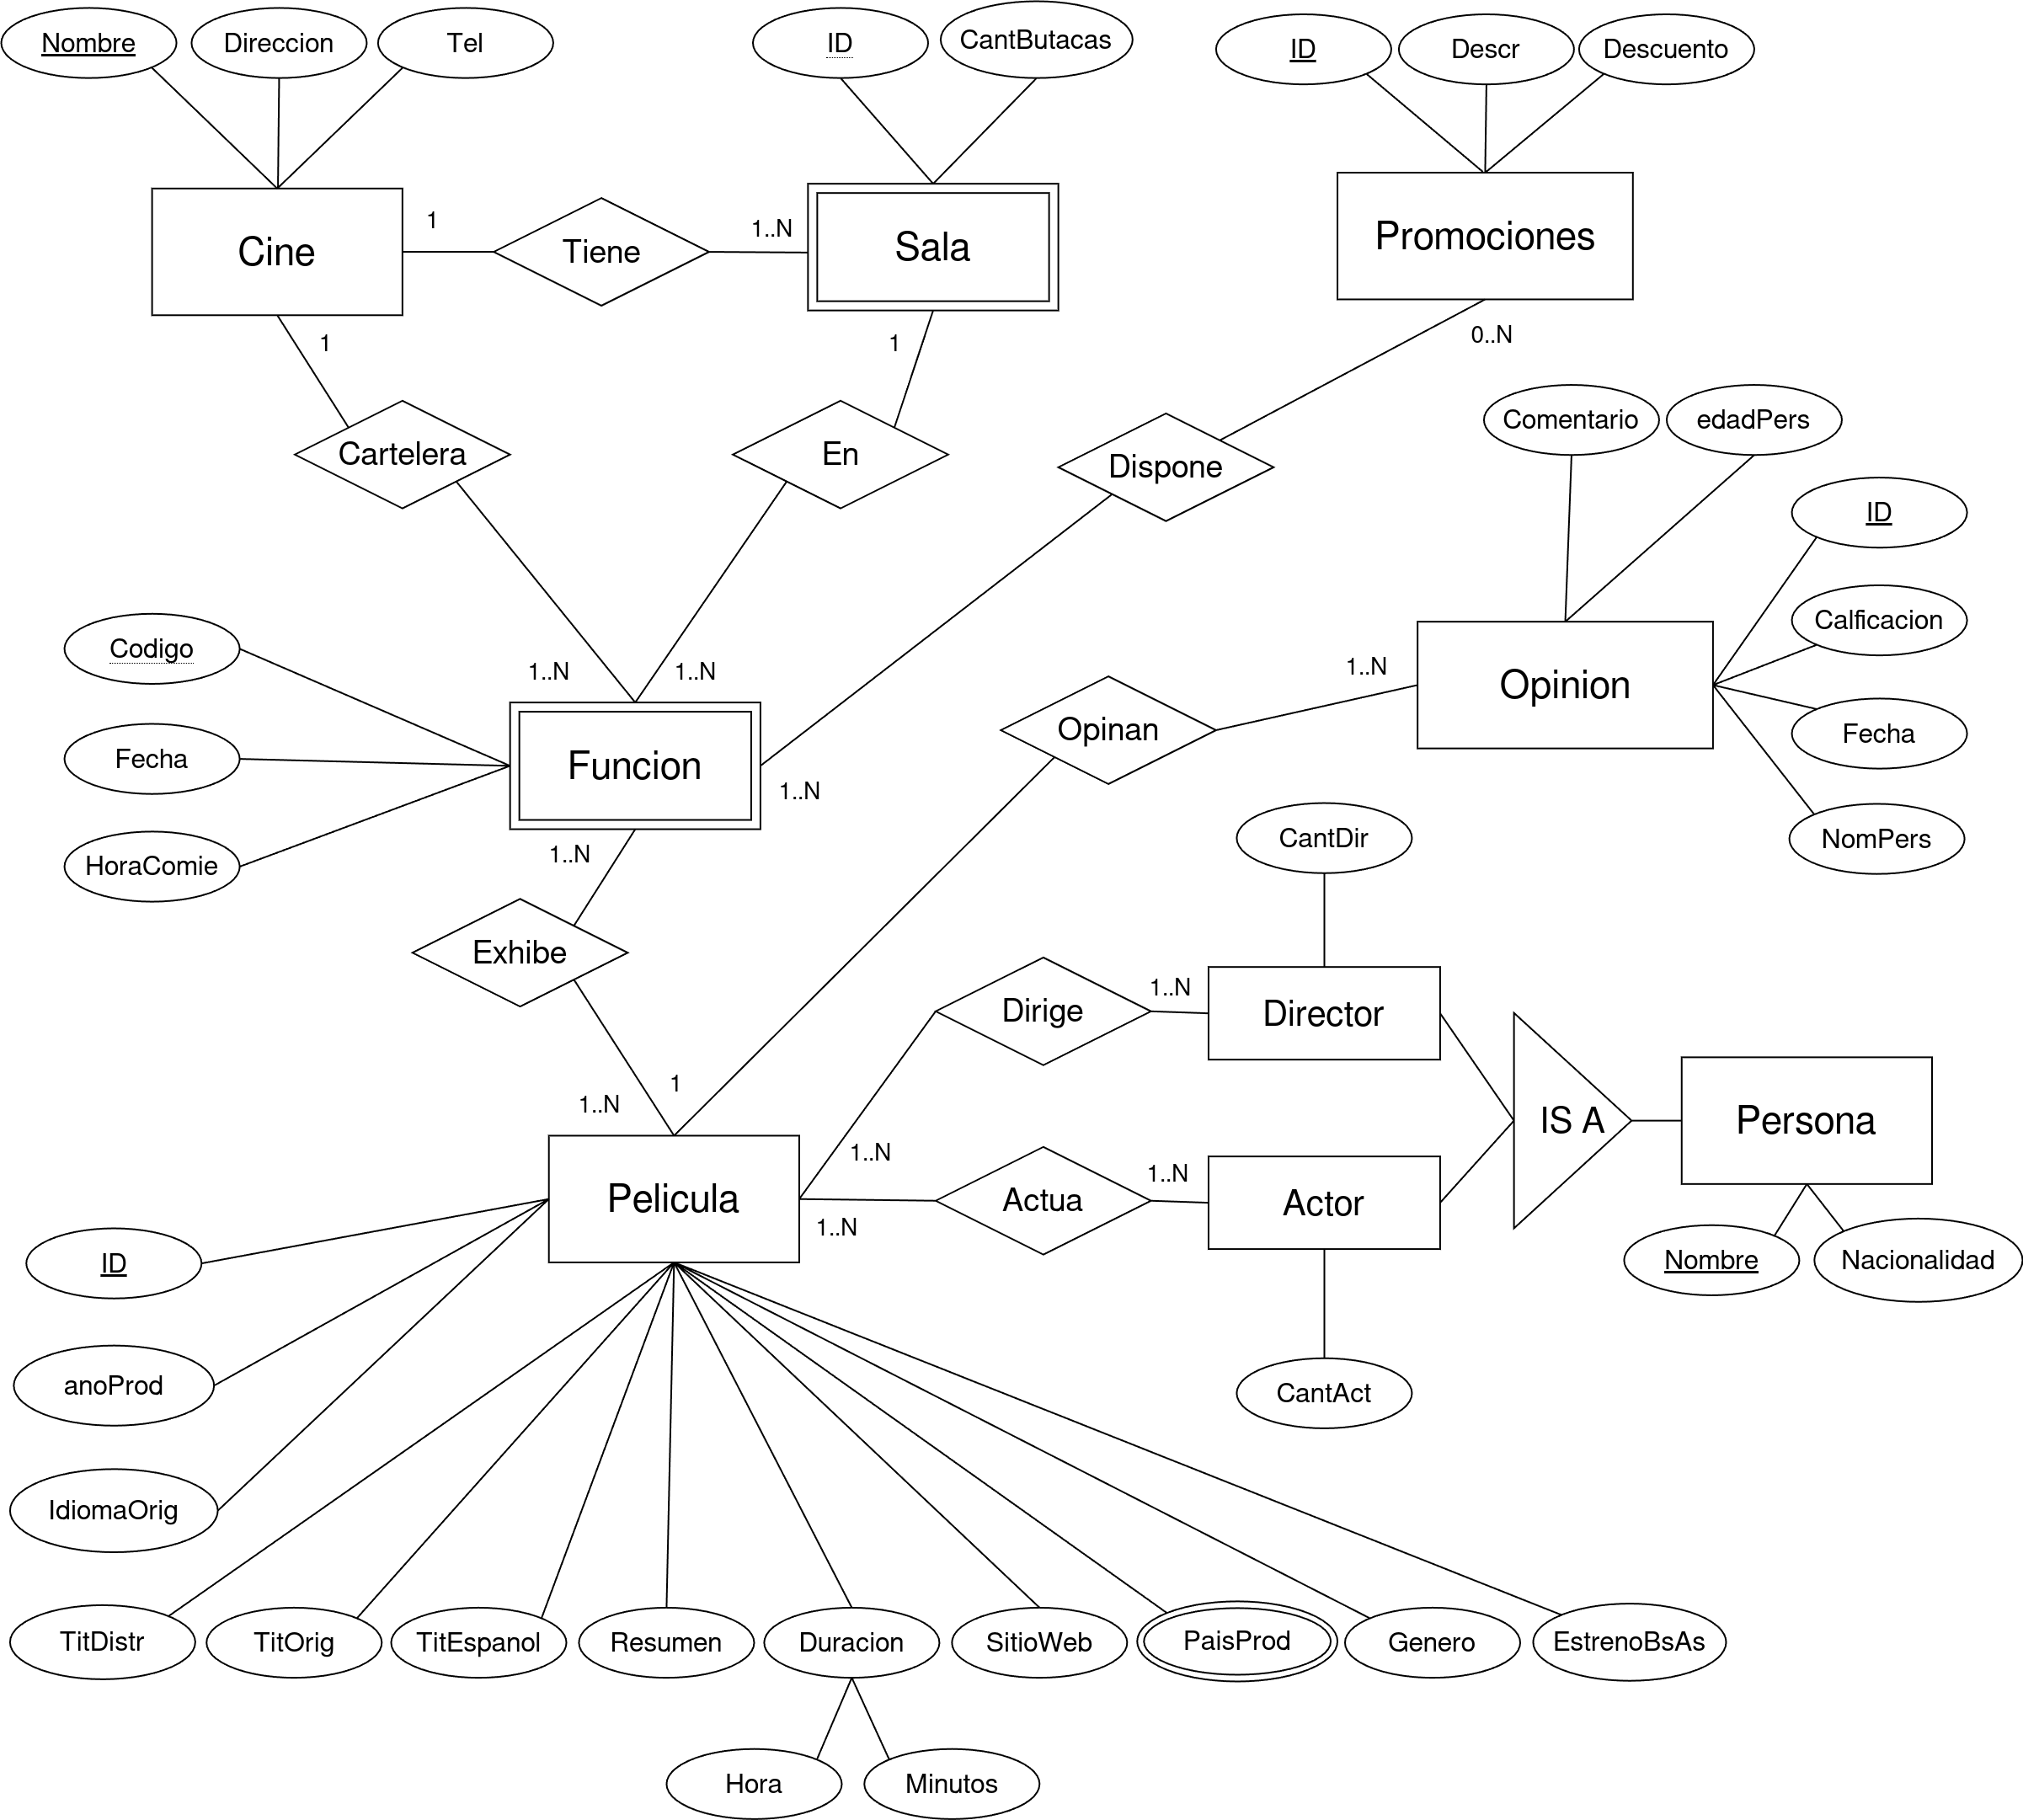
\includegraphics[scale=0.2]{Diagramm.png}
    \caption{Diagrama E-R.}
  \end{figure}

\section*{Modelo Relacional}
  \begin{enumerate}
    \item Cine(\underline{NomCine}, Direccion, Tel)
    \item Sala(\underline{IDSala}, \underline{NomCine}, CantButacas, NomCine) \newline
      NomCine CF a Cine
    \item Promocion(\underline{IDprom}, Descr, Descuento)
    \item Funcion(\underline{Codigo}, Fecha, HoraComie, NomCine, IDSala, IDpel) \newline
      NomCine CF a Cine, IDSala CF a Sala, IDPel CF a Pelicula
    \item Pelicula(\underline{IDpel}, añoProd, IdiomaOrig, TitDistr, TitOrig, TitEspañol, Resumen, DuracionHora, DuracionMinutos, SitioWeb, Genero, EstrenoBsAs, Calificacion)
    \item Opinion(\underline{IDopin}, Comentario, edadPers, Calificacion, Fecha, NomPers)
    \item Persona(\underline{NomPers}, Nacionalidad)
    \item Actor(\underline{NomPers}, CantAct) NomPers CF a Persona
    \item Director(\underline{NomPers}, CantDir) NomPers CF a Persona
    \item Actua(\underline{IDpel}, \underline{NomPers}) \newline
      IDPel CF a Pelicula, NomPers CF a Persona
    \item Dirige(\underline{IDpel}, \underline{NomPers}) \newline
      IDPel CF a Pelicula, NomPers CF a Persona
    \item Opinan(\underline{IDopin}, \underline{IDpel}) \newline
      IDopin CF a Opinion, IDPel CF a Pelicula
    \item Dispone(\underline{Codigo}, \underline{IDprom}) \newline
      Codigo CF a Funcion, IDprom CF a Promocion
    \item Posee(\underline{NomCine}, \underline{IDprom}) \newline
      NomCine CF a Cine, IDprom CF a Promocion
    \item PaisProd(\underline{IDPel}, \underline{Pais}) \newline
      IDpel CF a Pelicula
  \end{enumerate}

\section*{Dependencias Funcionales}

  \begin{itemize}
    \item Cine(\underline{NomCine}, Direccion, Tel)
      \begin{itemize}
          \item NomCine $\rightarrow$ Direccion, Tel
      \end{itemize}
      Por lo tanto esta en BCFN.
    \item Sala(\underline{IDSala}, \underline{NomCine}, CantButacas, NomCine)
      \begin{itemize}
          \item NomCine, IDSala $\rightarrow$ CantButacas
      \end{itemize}
      Por lo tanto esta en BCFN.
    \item Promocion(\underline{IDprom}, Descr, Descuento)
      \begin{itemize}
          \item IDprom $\rightarrow$ Descr, Descuento
      \end{itemize}
      Por lo tanto esta en BCFN.
    \item Funcion(\underline{Codigo}, Fecha, HoraComie, NomCine, IDSala, IDpel)
      \begin{itemize}
          \item Codigo $\rightarrow$ Fecha, HoraComie, NomCine, IDSala, IDpel
      \end{itemize}
      Por lo tanto esta en BCFN.
    \item Pelicula(\underline{IDpel}, añoProd, IdiomaOrig, ...)
      \begin{itemize}
          \item IDpel $\rightarrow$ añoProd, IdiomaOrig, ...
      \end{itemize}
      Por lo tanto esta en BCFN.
    \item Opinion(\underline{IDopin}, Comentario, edadPers, Calificacion, Fecha, NomPers)
      \begin{itemize}
          \item IDopin $\rightarrow$ Comentario, edadPers, Calificacion, Fecha, NomPers
      \end{itemize}
      Por lo tanto esta en BCFN.
    \item Persona(\underline{NomPers}, Nacionalidad)
      \begin{itemize}
          \item NomPers $\rightarrow$ Nacionalidad
      \end{itemize}
      Por lo tanto esta en BCFN.
    \item Actor(\underline{NomPers}, CantAct)
      \begin{itemize}
          \item NomPers $\rightarrow$ CantAct
      \end{itemize}
      Por lo tanto esta en BCFN.
    \item Director(\underline{NomPers}, CantDir)
      \begin{itemize}
          \item NomPers $\rightarrow$ CantDir
      \end{itemize}
      Por lo tanto esta en BCFN.
    \item 10-15 DMVs:
      \begin{itemize}
        \item IDpel $\twoheadrightarrow$ NomPers (Actua)
        \item IDpel $\twoheadrightarrow$ NomPers (Dirige)
        \item IDpel $\twoheadrightarrow$ IDopin (Opinan)
        \item Codigo $\twoheadrightarrow$ IDprom (Dispone)
        \item IDpel $\twoheadrightarrow$ Pais (PaisProd)
      \end{itemize}
      Por lo tanto esta en 4NF.
  \end{itemize}

\end{document}







  \begin{itemize}
    \item Cine(\underline{NomCine}, Direccion, Tel)
      \begin{itemize}
          \item NomCine $\rightarrow$ Direccion, Tel
      \end{itemize}
    \item Sala(\underline{IDSala}, \underline{NomCine}, CantButacas, NomCine)
      \begin{itemize}
          \item IDSala $\rightarrow$ NomCine, CantButacas \quad (si IDSala es globalmente único)
          \item NomCine, IDSala $\rightarrow$ CantButacas \quad (si IDSala es relativo al cine)
      \end{itemize}
    \item Promocion(\underline{IDprom}, Descr, Descuento)
      \begin{itemize}
          \item IDprom $\rightarrow$ Descr, Descuento
      \end{itemize}
    \item Funcion(\underline{Codigo}, Fecha, HoraComie, NomCine, IDSala, IDpel)
      \begin{itemize}
          \item Codigo $\rightarrow$ Fecha, HoraComie, NomCine, IDSala, IDpel
      \end{itemize}
    \item Pelicula(\underline{IDpel}, añoProd, IdiomaOrig, TitDistr, TitOrig, TitEspañol, Resumen, DuracionHora, DuracionMinutos, SitioWeb, Genero, EstrenoBsAs, Calificacion)
      \begin{itemize}
          \item IDpel $\rightarrow$ añoProd, IdiomaOrig, TitDistr, TitOrig, TitEspañol, Resumen,\\
          DuracionHora, DuracionMinutos, SitioWeb, Genero, EstrenoBsAs, Calificacion
      \end{itemize}
    \item Opinion(\underline{IDopin}, Comentario, edadPers, Calificacion, Fecha, NomPers)
      \begin{itemize}
          \item IDopin $\rightarrow$ Comentario, edadPers, Calificacion, Fecha, NomPers
      \end{itemize}
    \item Persona(\underline{NomPers}, Nacionalidad)
      \begin{itemize}
          \item NomPers $\rightarrow$ Nacionalidad
      \end{itemize}
    \item Actor(\underline{NomPers}, CantAct)
      \begin{itemize}
          \item NomPers $\rightarrow$ CantAct
      \end{itemize}
    \item Director(\underline{NomPers}, CantDir)
      \begin{itemize}
          \item NomPers $\rightarrow$ CantDir
      \end{itemize}
    \item PaisProd(\underline{IDPel}, \underline{Pais})
      \begin{itemize}
          \item IDpel $\twoheadrightarrow$ Pais
      \end{itemize}
  \end{itemize}
